\documentclass[10pt,conference,letterpaper]{IEEEtran}
\usepackage{times,amsmath,epsfig}
%
\title{XCPU2\\
Distributed Seamless Desktop Extension}
%
\author{%
{Latchesar Ionkov{\small $~^{\#1}$}, Eric Van Hensbergen{\small $~^{*2}$} }%
\vspace{1.6mm}\\
\fontsize{10}{10}\selectfont\itshape
$^{\#}$\,Los Alamos National Laboratory\\
Los Alamos, NM 87545, USA\\
LA-UR-09-02496\\
\fontsize{9}{9}\selectfont\ttfamily\upshape
$^{1}$\,lionkov@lanl.gov\\
\vspace{1.2mm}\\
\fontsize{10}{10}\selectfont\rmfamily\itshape
$^{*}$\,IBM Austin Research Laboratory\\
Austin, TX 78758, USA\\
\fontsize{9}{9}\selectfont\ttfamily\upshape
$^{2}$\,bergevan@us.ibm.com
}
%

\begin{document}
\maketitle
%

\begin{abstract}

XCPU2 is the evolution of our XCPU process management system 
which allows the users to compose the environment of the remote
cluster nodes to match that of their desktop workstation.  This
creates the illusion of cluster computation resources being a 
seamless extension of their desktop interface, facilitating 
cluster acceleration of workflows which can be composed and
visualized on the end-user desktop. 
XCPU2 allows programs running on the cluster to use 
the same versions of the libraries and tools the user installed 
locally on their desktop, and access support files such as configuration
and data in the familiar places in which they are located on the
end-user's workstation.

XCPU2 builds on our earlier work with the XCPU process management system. 
Like XCPU, XCPU2's interface is represented as a set of files
exported by a 9P file server. It supports heterogeneous clusters and
multiple head nodes. Unlike XCPU, it uses a pull instead of push model
for distributed applications, binaries, and data.

In this paper we describe the XCPU2 clustering model, its operation
and how the per-job filesystem configuration can be used to solve some
of the common problems when running a cluster.

\end{abstract}

\section{Introduction}

% emerging environment
Large scale cluster computing is becoming more and more mainstream
in today's environment.  Multiple vendors have introduced models for
offering computation as a service~\cite{ec2}~\cite{azure}~\cite{appengine},
providing on demand access to cluster computation resources for
dollars a day.  Additionally, hardware costs driven by economies of scale 
are increasingly favoring large clusters of low-cost, loosely coupled 
scale-out systems instead of comparatively expensive large scale-up 
SMP servers.  This sort of scale out configuration has been used in 
the realm of high performance computing (HPC) for many years.

A typical HPC cluster has a large number of compute nodes and a single
control/head node. They often use a parallel file system, that runs on 
a separate set of nodes, usually physically separated from the rest of the 
cluster. 
The control node is used to run the software that monitors the cluster 
health, the job scheduler that is used for scheduling and executing jobs 
as well as the compute node booting service. 
In most cases the compute nodes do not have
local disks, or if they do, they are only used for scratch space and don't
have an operating system installed. 
The compute nodes receive the operating system kernel and disk image over 
the network and store their file system in the node's RAM. 

In order to save memory and improve the boot time, 
system images are tens-to-hundreds of megabytes large and contain only the
most commonly used libraries and tools. Most of the cluster installations
support a single system image that is running on all compute nodes. Adding
new software, or upgrading the existing one is a complex task that requires
coordination between the cluster support group and all teams that use the
cluster. Upgrading a library required to run a new scientific code can take
weeks or months. The overhead and the time required for the coordination
makes it hard for groups to share clusters.

% desired user experience in this new era
The constrained nature of these cluster system images causes issues for
application developers who are used to developing code on a desktop or
workstation with a larger set of tools, scripting languages, and 
visualization tools which aren't available on the cluster.
End-users expect their cluster nodes to have the same environment 
as their local workstations including windowing systems, graphical 
integrated development environments (IDE), multiple scripting languages,
and a familiar file system and shell environment.  In many cases, end users
would prefer to be able to develop and launch jobs from their workstation,
and be able to use local tools and scripts to monitor and manipulate the
remote run.  They would prefer to be able to do all of this without
worrying about compatibility with the remote system image, using the 
cluster as a transparent computation accelerator.

% the unfortunate current state of affairs
In order to develop applications for the cluster, end-users are forced
to either use the same constrained software image on their workstation
or have a dedicated development server which matches the cluster configuration
to ensure that the application will execute correctly on the cluster.  While
the mainstream availability of virtualization tools have eased the pain of
maintaining separate development systems somewhat -- many end users are
unsatisfied with the limited software and tools in such environments.
Because the cluster environment differs so radically from their desktop
environment, it is difficult for developers to construct cohesive environments
which allows visualization and control to run locally while computation
runs remotely.  The result is most cluster systems resemble the same
batch-oriented runtimes which date back to card-punch-era computing instead
of the rich interactive visual environments many users have become accustomed
to on single node systems.

% plan 9 approach - maybe we want more here and less in related work?
The Plan 9~\cite{pike95plan} research operating system sought to address
these problems by creating a comprehensive approach to cluster 
computing which allowed organization of local and remote resources in
such a way that access to distributed resources (including computation)
was transparent.  Several years ago, LANL and IBM collaborated on v9fs
~\cite{graverobbers}, a port of the Plan 9 resource sharing protocol,
9P~\cite{9p}, to mainstream Linux.
LANL proceeded to bring Plan 9 style remote process management to UNIX
systems with their XCPU project~\cite{ron-xcpu}.

% opportunity overview
XCPU solved a portion of the cluster application environment problem
by identifying executable dependencies (such as dynamic libraries) and 
pushing them from the end-user node to the cluster nodes.  However,
non-executable dependencies such as scripts, configuration files, and
data were not automatically identified and would have to be present
on the cluster node's file system.  This problem was solved in Plan 9
through the use of the 9P resource sharing protocol coupled with Plan 9's
model of dynamic private namespaces~\cite{namespace}.  Recent additions
to the Linux kernel, including v9fs, bind mounts, and per-process 
private namespace~\cite{linuxns} present the opportunity to recreate this 
facility on mainstream Linux systems.

% paper summary
In this paper we introduce XCPU2, an evolution of our previous
XCPU work to provide a more complete execution offload mechanism
for Linux which is closer in capability to the Plan 9 based mechanisms.
XCPU2 allows the user to configure the view of the filesystem that will be
used when the job is run. It uses Linux support of private namespaces and
provides each job with its own filesystem view. XCPU2 allows parts of the
original filesystem to be ``bound'' to other locations and remote filesystems
to be mounted directly on the back-end cluster node. 
In the XCPU2 cluster model, the control node is used to
allocate nodes for a job, but the job control can be performed from any
other computer, including the user's desktop. In addition to controlling the
running job, the client-side tools export the filesystem of the controlling
computer, so it can be mounted and used by the compute nodes assigned for
the job. By using a filesystem configuration, all compute nodes can be
configured to have file system that is identical to the user desktop.

When a single application is run on multiple nodes, it is very likely that
the nodes will access the same files. All nodes will run the same
executable, use the same shared libraries and read the same configuration
files. Caching mechanisms that use that fact would have a much better
hit-to-miss ratio than the general-purpose ones. XCPU2 currently provides a
simple read-only hierarchical caching model in order to improve the performance.

In the next section we discuss related and past efforts dealing with cluster
execution frameworks.  Section 3 covers XCPU2's operation and interfaces.
We discuss our experiences deploying XCPU2 in section 4 and present a
performance evaluation in Section 5.  Section 6 contains our current
directions for future work and we conclude in Section 7.


\section{Related Work}

There are many process and resource management systems for clusters. In this
section we are going to describe the ones that influenced the development of
XCPU2, or are trying to provide the user with similar environment.

There have been attempts to make the cluster environment more flexible and allow
the users to pick from a limited set of system images. The current trend
is to use hypervisors on the compute nodes and create a cluster of
virtual machines that use the preferred system image. Another approach
requires rebooting the nodes assigned to a job with the requested image.
Both solutions cause some performance degradation due to additional
costs during startup.  
More problematic is that this multiplies the administrative
cost by the number of images a particular organization wishes to maintain.
Cluster image management solutions ~\cite{blutopia} and technologies
being developed for cloud computing ~\cite{mirage} may help with this to some extent, 
but the problem of matching a user's development environment on their Desktop 
persists.

The Beowulf Distributed Process Space (Bproc)~\cite{bproc} is a set of
Linux kernel modifications and user-space daemons that allows a user on the head
node to see the processes on all cluster nodes as local processes and
manipulate them with the standard Unix tools. Remote processes can be
examined, killed or debugged from the head node without any modifications of
the binary. The process view provided by Bproc is asymmetric, tools running
on the compute nodes still see only the local processes. That asymmetry as
well as the high cost of maintaining a Linux kernel patch outside of the
standard kernel distribution lead to exploring other more convenient solutions.

XCPU~\cite{ron-xcpu} is a process management system developed at LANL to
replace Bproc. The XCPU system consists of a daemon (XCPUfs) that runs on
each compute node, and a set of tools running on the head node. XCPUfs
creates a synthetic filesystem that can be mounted on Linux and Plan9, or
accessed via user space tools on other operating systems. 
Manipulation of the synthetic files allows
retrieving the state of the node, list of the processes or jobs running on
it and their running environment. The file interface also allows creation,
control and destruction of jobs. XCPU implements a push model: the
executable for the job is transferred from the head node to all compute
nodes explicitly. XCPU can push multiple files per job, so in addition to
the binary, it can also transfer all shared libraries it depends on,
and be manually configured to push configuration and data files 
required for the job's operation. On ELF
systems, like Linux and Solaris, XCPU can automatically detect and transfer
all shared libraries an executable depends on. This feature is very useful
on clusters with diskless compute nodes that are only using minimal OS
images. XCPU supports heterogeneous clusters automatically distributing the
appropriate binary for each architecture. The XCPUfs file hierarchy and
the operations performed on each file are described in details in
\cite{lucho-xcpu}.

XCPU's state is distributed across all compute nodes, each node keeping its
own state. If a control node crashes the rest of the cluster does not need to
be restarted, or any jobs canceled. All of the jobs can continue running
until the head node is rebooted. Once it is up, it collects the job
information and is in normal operation. Using file system interface also
allows more than one server to mount and control the compute nodes. That
feature allows configurations with hot-spare head nodes.

To improve the job startup time for large jobs, XCPU implements a
tree-spawn mechanism (Figure~\ref{fig:XCPU-tspawn}). The nodes assigned for
a job are organized in a tree, with the head node in the root, each node
having no more than adjustable number of children. The head node establishes
the process environment and transfers the required file to the nodes on the
first level of the tree. It then instructs them to \textsl{clone} their
state to their children. Once all nodes have their state set up, the head
node destroys the tree and starts the job execution.

\begin{figure}[h]
\begin{center}
\includegraphics[width=3in, keepaspectratio]{xcpu-tspawn.eps}
\end{center}
\caption{XCPU tree-spawn applied to a 12-node job, with 3 children per node.}
\label{fig:XCPU-tspawn}
\end{figure}

As mentioned previously, XCPU uses the 9P~\cite{9p} resource sharing protocol
originally developed for Plan9~\cite{pike95plan}.  It was chosen because 
of its simplicity and architecture independence as well as its ability to
access both control interfaces as well as normal files.

XCPU uses the standard Unix file permissions to ensure that the users only
start jobs to the nodes assigned to them. XCPUfs maintains a list of users
and groups. The ownership of the synthetic files and their read/write
permissions control what operations each user can perform on the node. In
addition to the user names and IDs, XCPUfs stores user's public key that is
used to ensure that the connection is established by the appropriate user.
The authentication scheme is similar to the one used in SSH2~\cite{rfc4252}.

XCPU2 borrows some ideas from Plan9's cpu~\cite{plan9-cpu} command. In Plan9
most of the OS and system services are represented as file trees. Operations
on devices and services are performed by normal read and write operations.
In Unix, most of these operations are performed using ioctl's, which by
their nature cannot be performed when the file is mounted on a remote
machine. In Plan9 all devices can be mounted and controlled remotely. The
cpu command uses this feature to reproduce on a remote server exactly the
same filesystem that the user has on his local machine. Because everything
is represented as files, a program running on a remote server that tries to
play a sound, will access the files that represent that are ``connected'' to
the user's local sound card. Using a simple resource sharing protocol and
the ``everything is a file'' concept, Plan9 solves many of the problems that
are being solved one piece at a time in Unix. The cpu command allows the
user to login to a remote server while seeing exactly the same file
namespace that was present on the local machine. The user experience when
using it is like ``importing'' the remote server CPUs and RAM to the local
machine -- everything else in his environment remains identical.

XCPU2 changes some important XCPU concepts. Instead of pushing the job
executable and supporting files explicitly, XCPU2 exports the file system
from the user's machine to all nodes assigned for the job. Using Linux
private namespaces, XCPU2 creates private view of the filesystem for each
job running on a node. XCPU2 allows that view to be configured depending on
the job and the cluster requirements. One of the commonly used file
namespaces is mimicking the cpu command behavior (as close as possible on
Linux) providing a view identical to the one on the user's machine.

\section{XCPU2 Operation}

\subsection{Computer roles}

XCPU2 recognizes three types (Figure~\ref{fig:XCPU2-nodes}) of computers
that participate in the job execution. The control node runs the tools
responsible for the cluster maintenance -- monitoring, resource management
and job scheduling. The compute nodes are assigned temporarily to a job and
run the user applications. Once the resource manager assigned a number of
compute nodes to a job, they are handed over to the job control machine,
which is responsible of preparing them for the job, running it, monitoring
and controlling its progress. Once the job finishes, the job control machine
hands the nodes back to the resource manager so they can be used by another
job. In some cases the control node is also used as a job control node.
In addition to that, XCPU2 allows the user desktop, or any other computer to
serve that role.

\begin{figure}[h]
\begin{center}
\includegraphics[width=3in, keepaspectratio]{xcpu2-nodes.eps}
\end{center}
\caption{XCPU2 computer roles}
\label{fig:XCPU2-nodes}
\end{figure}

\subsection{Compute node daemon}

XCPUfs is the XCPU2 daemon that is running on each compute node. It exports
its interface as a file tree. XCPUfs maintains a list of users that can
attach to the interface and perform process management operations remotely.
XCPUfs is implemented as a user space 9P file server and can be accessed
over the network using any 9P client software.

\subsubsection{XCPUfs authentication}

Unlike other network file protocols, 9P requires each user to authenticate
to the server explicitly. Before an user can perform any operations, it
needs to authenticate itself to XCPUfs. The daemon allows two authentication
mechanisms. The first one is similar to the challenge-response
authentication used in SSH2. XCPUfs sends a challenge string, the client
signs it with the user's private key, and the daemon verifies the signature
using the user's public key. When the user is already authenticated, he can
read a \textsl{passkey} from the \texttt{passkey} file. The passkey can be
stored or transported to another server and used later to authenticate as
the same user. Each passkey can be used only once.

\subsubsection{XCPUfs sessions}

XCPU2 allows more than one job running on a compute node at the same time. A
job is comprised of many XCPUfs \textsl{sessions} running on multiple
nodes. Each session defines a single program that is run on a single node as
a part of the job. The session defines program's environment, its arguments,
the filesystem view as well as the name of the program to run. Once the
program is running, the user can send data to its standard input, read its
standard output or error streams, or send signals. When the program
terminates, the user can read program's exit code.

Each session on the node is represented as a directory that contains the
files used to control it. Table~\ref{tbl:XCPU2-session} lists the session
files and their purpose.

\begin{table}[ht]
\begin{center}
\begin{tabular}{lp{2.4in}}
    Name & Description\\
    \hline
    \ttfamily ctl & Session control file\\
    \ttfamily argv & Program arguments\\
    \ttfamily env & Program environment variables\\
    \ttfamily stdin & Standard input stream\\
    \ttfamily stdout & Standard output stream\\
    \ttfamily stderr & Standard error stream\\
    \ttfamily wait & Exit code. Reading blocks until program termination\\
    \ttfamily id & Job ID (set by the client)\\
    \ttfamily ns & Session namespace\\
\end{tabular}
\caption{Session files}
\label{tbl:XCPU2-session}
\end{center}
\end{table}

A new session is created by opening the top-level \texttt{clone} file. The
open operation creates a new session and its corresponding directory.
Reading from the opened \texttt{clone} file returns the session ID, which is
the same as the session directory name. The session directory remains
accessible as long as there is at least one file in it that is open, or
until the program associated with the session is running. Once the program
terminates and all session files are closed, XCPUfs destroys the session and
releases all resources it used.

\begin{table}[ht]
\begin{center}
\begin{tabular}{lp{1.9in}}
    Command & Description\\
    \hline
    exec \textsl{filename} & Execute the program. Can be used only once\\
    wipe & Kill the program if running and destroy the session\\
    signal \textsl{signame} & Send signal to the running program\\
    close std{\ldots} & Close the specified standard stream\\
    redirect std{\ldots} \textsl{file} & Redirect the standard stream from/to the file\\
    id \textsl{ID} & Set session job ID\\
\end{tabular}
\caption{Session commands}
\label{tbl:XCPU2-sctl}
\end{center}
\end{table}

Session's \texttt{ctl} file is used to control the session state. By writing
commands, the user can change its state -- start the program execution, send
signals to the program main process, close or redirect the program standard
streams. A command starts with the command name, followed by a number of
arguments separated by the space character, and ends with a new-line
character. Table~\ref{tbl:XCPU2-sctl} shows the list of session commands
supported by XCPUfs.

In order to provide support for multiple head nodes, XCPUfs ensures that all
readers from \texttt{stdout} and \texttt{stderr} receive all the data. 

\begin{table}[ht]
\begin{center}
\begin{tabular}{lp{1.9in}}
    Command & Description\\
    \hline
    unshare & Create private file namespace for the session\\
    mount \textsl{dev} \textsl{dir} \textsl{type} \textsl{options} & Mount a filesystem\\
    bind \textsl{olddir} \textsl{newdir} & Bind a subtree from the filesystem to another place \\
    import \textsl{addr} \textsl{dir} & Mount a 9P filesystem\\
    cd \textsl{dir} & Change the current directory\\
    chroot \textsl{dir} & Make \textsl{dir} the root of the filesystem\\
    cache \textsl{addr} & Cache the content of the 9P filesystem locally\\
\end{tabular}
\caption{Namespace commands}
\label{tbl:XCPU2-ns}
\end{center}
\end{table}

The \texttt{ns} file contains a list of instructions on how to build the
session's filesystem namespace before running the program. XCPUfs allows the
session to create its private namespace by using the \textsl{unshare}
command. Once it is specified, all changes to the filesystem (mounts and
binds) are private to the processes that belong to the session, and are not
visible to the rest of the processes running on the node. The namespace file
can contain references to environment variables defined for the session. The
references are replaced with the environment values before the namespace
commands are executed. Table~\ref{tbl:XCPU2-ns} shows all commands that can
be used for the namespace definition. The default session namespace is
defined as:

\begin{verbatim}
  unshare
  import $XCPUTSADDR /mnt/term
  bind /mnt/term/$XCPUARCHDIR /mnt/sandbox
  bind /mnt/term/home /mnt/sandbox/home
  bind /dev /mnt/sandbox/dev
  bind /proc /mnt/sandbox/proc
  bind /sys /mnt/sandbox/sys
  chroot /mnt/sandbox
\end{verbatim}

After creating the private namespace, XCPUfs mounts the filesystem exported
by the job control node (contained in the XCPUTSADDR variable), binds the
directory that contains the files for the compute node architecture, binds
the local \texttt{/dev}, \texttt{/proc} and \texttt{/sys} directories at the
appropriate places and makes \texttt{/mnt/sandbox} the root directory of the
namespace. This in effect hides the node's local filesystem from the
program, providing the same filesystem view that it would have if running on
the job control node.

\subsubsection{Top-level files}

The synthetic files on the top level of the XCPUfs file tree are used for
operations common to all sessions. Table~\ref{tbl:XCPU2-top} lists their
names and description.

\begin{table}[ht]
\begin{center}
\begin{tabular}{lp{2.4in}}
    Name & Description\\
    \hline
    \ttfamily clone & Create new session\\
    \ttfamily ctl & Node control file\\
    \ttfamily arch & Node's OS and CPU architecture\\
    \ttfamily env & Default session environment\\
    \ttfamily procs & Process list\\
    \ttfamily state & State of the node (set by the client)\\
    \ttfamily passkey & Generate a new passkey for authentication\\
    \ttfamily pwent & List of users\\
    \ttfamily grent & List of groups\\
    \ttfamily ns & Default session namespace\\
\end{tabular}
\caption{Top-level files}
\label{tbl:XCPU2-top}
\end{center}
\end{table}

The \texttt{env} and \texttt{ns} files allow the cluster administrator to
set the default values for all sessions created on the node. When a new
session is created, the initial values of its environment and namespace are
copied from the top-level files. The \texttt{procs} file contains a list of
all processes running on the compute node. The list is represented in
S-expression with first line defining the entries that are returned for each
process. The top-level \texttt{ctl} file accepts commands in the same format
as the session \texttt{ctl} file.

User and group management is performed by using \textsl{user-add},
\textsl{user-del}, \textsl{group-add}, \textsl{group-del},
\textsl{user-add-group} and \textsl{user-del-group} commands. Each user
group has a name, group ID and a list of members. The users have name, ID,
default group and a public key that is used to authenticate them. XCPUfs
defines a special group and user ``XCPU-admin'' with ID 65530. Initially all
XCPUfs files are owned by XCPU-admin, so that is the only user that can add
other users. The admin can change the ownership and permission of any file 
using chown and chmod commands. If an user can write to the \texttt{ctl}
file he can add or delete users, kill processes etc. If an user is granted
permission to read from the \texttt{clone} file, he can create new sessions
and run programs on the node.


\subsubsection{Examples on using standard Unix tools to perform XCPUfs
operations}

Assuming that the XCPUfs filesystem is mounted on /mnt/XCPU, the user can:

Add a new user:

\begin{verbatim}
  echo user-add glenda 500 mammals \
    `ssh-rsa AAA...Sw== glenda@lanl.gov' \
     > /mnt/XCPU/ctl
\end{verbatim}

Kill process with PID 432 on the node:

\begin{verbatim}
  echo kill 432 > /mnt/XCPU/ctl
\end{verbatim}

Create a new session and set the program arguments:

\begin{verbatim}
  tail /mnt/XCPU/clone &
  12
  echo foo bar then > /mnt/XCPU/12/argv
\end{verbatim}

\subsection{Job Control Tools}

The job control node and the compute nodes act both as 9P servers and
clients. The job control node is a client for the XCPUfs file servers
running on the compute nodes. It is also a 9P server that exports the
control node's file system over 9P. The compute nodes are 9P clients
mounting the job control node filesystem and are also 9P file servers
that export XCPUfs process control interface over 9P.

Although most of the XCPU2 operations can be performed by mounting the
XCPUfs file interface on the job control node and reading and writing from
its files, it is not always convenient for the users to do so. XCPU2
provides a library that provides a C interface for creating and manipulating
jobs, users and sessions. Mounting a filesystem in Unix requires root
privileges on the job control node. In order to provide more flexibility,
the libXCPU library doesn't depend on mounting the file system. Instead, it
uses a 9P client library to perform all I/O operations from user space.
LibXCPU is used to implement the standard XCPU2 tools as well as integration
with third-party services, like mpich and mvapich. XCPU2 provides tools for
running a job (xrx), user (xuserset) and group (xgroupset) management,
process enumeration (xps) and control (xk).

XCPU2 uses the standard SSH2 RSA public key located in \$HOME/.ssh for
authentication.

\subsection{Cache implementation}

When XCPU2 is used, the programs for a job on all compute nodes ``see'' the
same filesystem that the user sees on the job control node. The convenience
comes with the price that the job control node, or the user desktop, may
become a bottleneck. Accessing the same file server from all compute nodes
is not going to scale well when scaling the job. 

Normally a job runs the same executable on all nodes. The executable depends
on the same shared libraries, reads the same configuration file and uses the
same data. It makes sense for all node for a job to participate in some type
of cooperative caching scheme. And because XCPU2 is responsible for building
the namespace and controlling the job, it is convenient to include the cache
in XCPU2. 

Currently XCPU2 implements a simple cooperative cache scheme that is best
suited for sharing systems, read-only files. It doesn't ensure cache
coherence and modifications on one compute node are not propagated to the
job control node, or other compute nodes. The cache scheme is similar to
XCPU's tree-spawn mechanism. XCPUfs makes the caching filesystem as part of
the file tree it exports. When the job starts, the nodes are organized in
a tree with the job control node in the root. On each node, the caching file
server connects to its parent's caching filesystem. The local caching file
server is mounted as the root filesystem for the program running on the
compute node. When the program tries to access a file, the caching file
server checks if the file is already present locally. If not, it contacts
its parent caching file server and requests the file. Once it receives the
file it stores it locally, and all subsequent requests for the file are
fulfilled using the local copy. Because all nodes are going to use the same
files, it is very likely that the parent already has a copy of the file, or
if not, that after copying it from the parent's parent the file will be
requested from the other children and used locally.

\begin{figure}[h]
\begin{center}
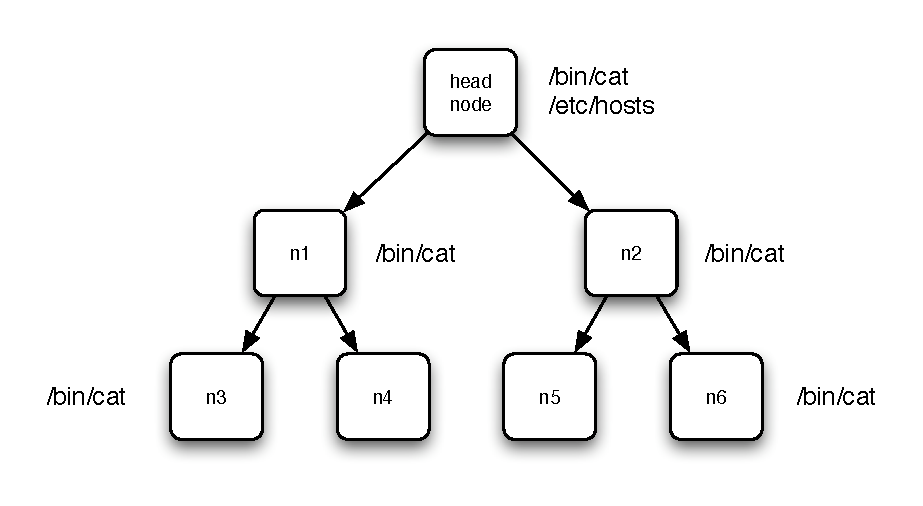
\includegraphics[width=3in, keepaspectratio]{xcpu2-cache.eps}
\end{center}
\caption{XCPU2 caching file server}
\label{fig:XCPU2-cache}
\end{figure}


Figure~\ref{fig:XCPU2-cache} shows an example of the caching scheme. If the
job runs the command \texttt{cat /etc/hosts}, node n3 will try to read and
execute the file \texttt{/bin/cat}. The caching file server will try to read
it from its parent n1. N1 doesn't have it locally, so it will request it
from the job control node, save it locally and send it to n3. Microseconds
later n3 itself will need to run \texttt{/bin/cat} but because the file is
stored locally it doesn't have to request it from its parent again. When n4
accesses the file, its parent will have it locally and won't go all the way
up to retrieve it.

The scheme scales well with the size of the files, but has some major
drawbacks. It cannot be used for files that are modified in one or more of
the compute nodes. It also doesn't use the local storage efficiently storing
the same data on multiple nodes. In future, we are planning to implement a
more efficient caching scheme.

\section{Case Studies}

%
% I realized that I may get flak for talking about this because it was vaguely
% product, but never really materialized.  Fortunately the customer talked about it
% http://www.prace-project.eu/hpc-training/prace-winter-school/Carteni_PRACE_WS.pdf
% So we should probably cite that
%


\subsection{Virtual�PowerXcell�Environment�(VPE) Hypernodes}

Roadrunner~\cite{roadrunner}, the world's first petascale supercomputer, was 
architected as a hybrid system composed of general purpose Opteron processors 
with Cell-based accelerators.  
Roadrunner's success led to interest in smaller scale and more loosely coupled
hybrid clusters.
The Virtual PowerXcell Environment (VPE) was the underlying runtime of a prototype
hybrid blade cluster made up of hypernodes.  Each hypernode consisted of a Power 6 
blade (JS22) acting as general purpose front-end to a number of back-end PowerXcell 
blades (QS22) acting as compute accelerators connected over a high-performance 
Infiniband network.

The intent of the hypernode systems software environment was to maintain the
illusion of a tightly coupled single system even though the applications were running 
on a loosely coupled cluster.  In order to accomplish this we specially tagged hybrid 
applications with a custom header identifying them as VPE executables.  
We then built a custom binfmt~\cite{binfmt} module which would recognize the 
VPE header and transparently reserve cluster resources using a workload scheduler 
and use Xcpu2 to schedule the execution of the application on the remote node 
using the front-end nodes environment and operating system.  With the console 
redirected to the same terminal which initiated the execution, environment
variables duplicated and signals forwarded, the user is unaware that the 
application is even running on a remote system.  
The nature of this execution model is such that there is a one-to-one correlation
between the proxy application on the front-end node and the instance running on the
back-end cluster node.  The implication is that we can't take much advantage of the
treespawn or caching mechanisms provided by XCPU2 when fanning out computation to
many back-end nodes.
This transparent remote execution mechanism was originally developed as part of the 
PROSE LibraryOS project~\cite{prose}~\cite{libra}.

The hypernode file system environment was maintained by a GPFS~\cite{gpfs} cluster which
was mounted on the front-end JS22 nodes.
The PowerXcell blades were configured as diskless drone systems
and booted with a minimal ramdisk containing only enough resources to establish
themselves as Xcpu2 servers.  All application executables and data were obtained
by the QS22s via the 9P connection to the JS22 front-end established by Xcpu2.
This configuration had the effect of aggregating file system access by the QS22's 
through the JS22 (in much the same way BlueGene compute nodes aggregate file
access through their I/O nodes~\cite{bgp}) allowing a more simple configuration 
environment,  and an extremely small systems software footprint on the QS22 nodes.

One unforeseen complication of our transparent distributed execution model
was in dealing with intelligent runtimes who optimize their communication
based on thread location.  For example, when we ran MPI applications in a
VPE environment we could convince MPI to start extra threads to be scheduled
on the remote nodes, but since it thought those threads were running locally it
would try to use shared memory for communication between them.  Since
memory is not one of the resources shared between front-end and back-end nodes
this caused our naive configuration of the MPI application to fail.  With some
effort we were able to identify an MPI library version and configuration which
would allow us to override the shared memory communication optimizations.

Another issue we had was trying to do proper resource allocation of the back-end
accelerators.  Each QS22 PowerXcell blade had 16 synergistic processing units~\cite{ibm-cell}
(SPUs) which applications could use.  Because these accelerator resources were not
accounted for via the Xcpu2 file server, we had no integrated mechanism to monitor
or reserve SPUs for a particular applications and had to resort to a third-party resource 
reservation system which the applications had to interact with directly.  We will discuss
some ideas of how to address this in the future work section.


\subsection{The Pinkish development cluster}

Pinkish is the 91-node cluster the system's research team at LANL uses for
development and testing. The compute nodes use coreboot~\cite{coreboot}
instead of a standard BIOS and load the OS kernel and system image over the
Myrinet network using XGet~\cite{xget}. The root filesystem on the compute
nodes contains only few system commands (implemented by busybox), shared
libraries and xcpufs and xcpufs2 daemons.

In addition to the head and compute nodes, we have a number of other
servers connected to the same network running various Linux distributions.
XCPU2 allows us to quickly simulate a particular configuration on all
compute nodes and test for any scalability issues of the software we are
working on. Normally we use a namespace that mounts the distribution's root
filesystem via XCPU2's cache file server. The user directories are mounted
from pinkish head node over NFS and we use tmpfs for temporary files on the
nodes.

This configuration is what was used to obtain the performance results
in the next section.


\section{Performance}

We used our development cluster, pinkish, to compare the XCPU2 performance
with XCPU and pdsh. The pinkish cluster has 91 nodes with dual Opteron
processors, 2GB of RAM, and a 2Gb/s Myrinet interconnect.

\begin{figure}[h]
\begin{center}
\includegraphics[width=3in, keepaspectratio]{results1.eps}
\end{center}
\caption{Comparison of the performance of XCPU, XCPU2 and pdsh-ssh when
executing 1MB binary (2.93MB including the shared libraries).}
\label{fig:XCPU-results1}
\end{figure}

Figure~\ref{fig:XCPU-results1} compares XCPU, XCPU2 and pdsh (with its ssh
plugin) results when running a different job sizes. Pdsh doesn't transfer
the binaries to all nodes, only starts and controls the program execution.
In order to achieve reasonable comparison, for the pdsh test as a part of
the run we mount the head node's root filesystem on the compute nodes,
\textsl{chroot} it so it is a root filesystem for the job, execute the
binary, then unmount the NFS server. This ensures that, like XCPU and XCPU2,
the nodes transfer the binary and the shared libraries from the head node.
The XCPU2 performance is close to the XCPU one and the small performance
penalty is justified by the improvements in the user experience.

\begin{figure}[h]
\begin{center}
\includegraphics[width=3in, keepaspectratio]{results2.eps}
\end{center}
\caption{Performance of the XCPU tree-spawn mechanism to the XCPU2 caching
file server when executing 1MB binary (2.93MB including the shared
libraries). Both methods are configured so the tree has no more than 8
children per parent.}
\label{fig:XCPU-results2}
\end{figure}

Figure~\ref{fig:XCPU-results2} compares the XCPU tree-spawn mechanism to
XCPU2 caching file server. The results show that with the increase of the
job size, the current XCPU2 caching implementation doesn't scale as well as
XCPU. One of the reason's for that behavior might be the fact that the
current caching mechanism transfers the whole file from the parent node
before it starts serving requests for that file. The asynchronous
file transfer implementation in XGet is one of the approaches we might try
in future to improve the cache file server.

\begin{figure}[h]
\begin{center}
\includegraphics[width=3in, keepaspectratio]{results3.eps}
\end{center}
\caption{Comparison of XCPU2 with or without the caching scheme.}
\label{fig:XCPU-results3}
\end{figure}

Figure~\ref{fig:XCPU-results3} shows the results when running XCPU2 with
flat vs. tree-like caching file server. We tested binaries with various
sizes on 64 of the cluster nodes. The results show that using hierarchical
cache tree scales much better than a flat caching.

We need to perform further performance testing on larger clusters in order
to evaluate XCPU2 scalability and changes that can improve it.

\section{Future work}
%
% This is pretty rough, and I'm pretty much coming up with it as I go
% maybe we'd be better off just stating the problem (and incorporating
% the problem of virtual machines and cloud environments as well).
% I may take a second pass at this once I've had a chance to sleep on it.
%

Emerging hybrid computing models such as NVIDIA's 
CUDA~\cite{cuda}, the Roadrunner supercomputer, and the PowerXcell hypernodes
require additional support from the XCPU environment to support resource 
reservation, monitoring, and control.  Some early attempts ~\cite{cellfs} have been
made to extend synthetic file system control and monitoring of such environments
-- but it is our belief that a more tightly integrated model would benefit clusters in
which such hybrid accelerators are present.

Such additional facilities may be provided by synthetic file system plug-ins.  The
naturally extensible nature of synthetic file system hierarchies should allow these
hybrid systems and their control interfaces to co-exist with more conventional
environments.  In this way, monitoring utilities and job schedulers can have a
single interface to obtain information about all aspects of the hybrid system.  A
similar approach could be taken for virtual environments, deepening the hierarchy
of control interfaces to allow control interfaces for the node, virtual  machine instance,
and associated accelerators.

The XCPU and XCPU2 model both take a broadcast approach to standard I/O -- 
that is to say that stdin is replicated and broadcast to all remote threads of a 
session and stdout response is aggregated back to the initiating thread.
This works great for many applications where standard I/O is primarily used
for monitoring, but emerging cluster environments ~\cite{push} may wish to
choose different options.  For example, XCPU2 could be used to fan-out
worker nodes for map/reduce type problems.  In such scenario's standard I/O
could be used to issue unique instructions to each worker node and gather 
responses -- or it may even be desirable to route standard out from one worker
node to another.  Extending XCPU2 to allow the use of standard I/O as per node
communication paths would facilitate such environments.   Additional
communication channels could be brokered, perhaps even for inter-worker
communication obviating the need for additional message passing infrastructure.

The use of the unshare system call, together with bind operations limits XCPU2
operation to Linux or Plan 9 back-end systems.  Such facilitates do not currently
exist on other operating systems such as MacOSX, BSD, or Windows.  One
possibility would be to use an intermediary who could compose dynamic 
private namespaces and export the pre-composed namespace to the operating
system providing the XCPUfs service.  Private namespace could be provided by
chrooting to a sandbox based on this pre-composed namespace.
% Does windows have the concept of a chroot?
The hosted version of the Inferno operating system has sufficient functionality
to provide this service on a variety of platforms, and could export the precomposed
namespace as a 9P file system which could be mounted by MacFUSE or v9fs.
This could also open up the opportunity of using Inferno-based authentication
servers and encryption technologies which would further secure the environment.

An obvious area for improvement are optimizations in data flow.  While we
support caching accessed elements of the user's file system within the 
cluster, often times the user is actually accessing data in a parallel file
system which is mounted on both his desktop and the cluster.  In this
scenario routing all file system traffic through his desktop node becomes
a bottleneck.  This scenario can be overcome with proper manipulation of the
namespace configuration, however it is desirable for the system to be able
to automatically identify and optimize for such transitive file system
mount operations.

Furthermore, since many of the nodes within the cluster will be caching
similar data, a peer-caching policy where nodes check with their peers 
before going to the file system origin is also desirable.  Configuration
for this sort of scenario will likely be tightly coupled to the topology of
the underlying high performance interconnect.  In order to ease administration,
it would be desirable if characteristics of the high performance interconnect
could be discovered by the system instead of explicitly defined by the end
user.

A less performance critical aspect of the cluster configuration is the 
initial node discovery process.  XCPU2 still relies on static configuration
files for identifying members of the cluster.  A more dynamic environment
with autodiscovery and configuration using zeroconf~\cite{zeroconf} would
greatly simplify creation of ad-hoc clusters.  Provisions for hierarchical
discovery would also be nice to accommodate environments with multiple hidden
levels of network (such as systems behind NATs, alternate network gateways, 
etc.)

Such richer network environments will also require a change to how XCPU
servers mount the client's environment.  Right now, a back-mount is 
initiated through the namespace file.  In order to traverse network
boundaries and barriers such as NAT devices cleanly, it would be preferable
for a single connection to be used to both initiate computation and provide
the reverse mount.  This is the method used by the Plan 9 cpu(1) and Inferno
rcmd(1) mechanisms.


\section{Conclusions}

% recap
As cluster computing becomes more and more of a mainstream environment, it
is critical that we develop tools which maximize its potential by seamlessly
integrating distributed resources with the end-user's desktop environment.
By providing computation on demand we can create a more efficient and effective
work environment for solving academic, commercial and high-performance 
computing problems.
In this paper we have discussed the ongoing evolution of the Xcpu2 
framework for enabling this model of computation offload for application
acceleration.  We describe how it addresses shortcomings of its predecessor,
and lay out ideas for its future development.
Xcpu2 continues to evolve, we encourage you to try it for yourself and
participate in its development.  The current version is open source and
available along with its Xcpu predecessor at http://xcpu.org.

\section*{Acknowledgements}

Aspects of this work originating at IBM have been supported by the
Department of Energy under Award Number DE-FG02-08ER25851.

The work at LANL was done as part of the Usable Supercomputer project which
is funded by the NNSA's Advanced Simulation and Computing Program.


\bibliographystyle{IEEEtran}
\IEEEtriggeratref{18}
\bibliography{xcpu2}

\end{document}
